% -*- coding: UTF-8 -*-
% vim: autoindent expandtab tabstop=4 sw=4 sts=4 filetype=tex
% vim: tw=72
% vim: spelllang=de spell
% chktex-file 27 - disable warning about missing include files

\subsection{Ray Casting}
\label{subsec:ray_casting}

\textit{Ray Casting} ist ein Verfahren zur Simulation, wieviel Licht
anhand eines (Licht-) Strahles zu der sichtbaren Bildfläche (also dem
Betrachter) transportiert wird.

Das Verfahren wurde erstmals
in~\citetitle{appel_techniques_1968}~\citeyear{appel_techniques_1968}
von~\citeauthor{appel_techniques_1968} vorgeschlagen und
auch~\citeyear{arlington_mathematical_applications_group_inc_afips_1968}
von
der~\citeauthor{arlington_mathematical_applications_group_inc_afips_1968}
in~\citetitle{arlington_mathematical_applications_group_inc_afips_1968}
erfolgreich umgesetzt.

Ein möglicher Algorithmus, wie Ray Casting umgesetzt werden kann, findet
sich in~\autoref{fig:ray_casting:high_level}.

Bei dem Ray Casting Verfahren wird ein \textit{Projektionszentrum} (das
Auge eines Betrachters) sowie eine Region einer beliebigen Bildfläche
gewählt. Dabei kann die Region als gerasterte Fläche angenommen werden.
Jedes Raster entspricht den Bildpunkten (Pixeln) der gewünschten
Auflösung. Je feiner die Rasterung, desto höher die Auflösung.

Für jeden Bildpunkt der gewählten Region wird ein Strahl generiert,
welcher dann vom Projektionszentrum durch das Zentrum des Bildpunktes
auf die Szene ``geworfen'' wird. 

Es wird dann das Objekt gesucht, welches den nächsten Schnittpunkt mit
dem Strahl bildet. Für jede Lichtquelle der Szene wird geprüft, ob die
Lichtquelle vom Schnittpunkt aus sichtbar ist. Ist dies der Fall, wird
schliesslich die Farbe und die Intensität der Farbe an diesem Schnittpunkt
anhand eines Beleuchtungsmodelles (z.B.\ dem Phong-Beleuchtungsmodell)
berechnet. Andernfalls befindet sich der Punkt im Schatten, er wird also
nicht beleuchtet.

\begin{figure}[H]
    \centering
    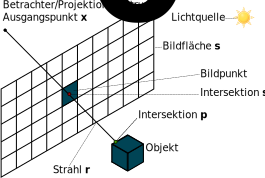
\includegraphics{img/ray_casting.pdf}
    \caption{Illustration des Ray Casting Verfahrens\protect\footnotemark}\label{fig:ray_casting_illustration}
\end{figure}
\footnotetext{Eigene Darstellung mittels Inkscape}

Die obenstehende~\autoref{fig:ray_casting_illustration} zeigt das
Prinzip des Ray Castings. Ausgangspunkt bildet der Betrachter mit $x_{0}
= (x_{x_{0}}, y_{x_{0}}, z_{x_{0}})$. Es wird ein Strahl $r = (x_{0},
d)$ in Richtung $d$ der Bildfläche $s$ ``geworfen''. Der Strahl $r$
schneidet die Bildfläche $s$ an einem Punkt $sp = (x_{sp}, y_{sp},
z_{sp})$.  Somit ergibt sich die Richtung des Strahles $d = sp - x_{0} =
(x_{sp} - x_{x_{0}}, y_{sp} - y_{x_{0}}, z_{sp} - z_{x_{0}}) = (x_{d},
y_{d}, z_{d})$. Der Strahl $r$ trifft und schneidet schliesslich ein
Objekt am Punkt $p = r(t) = x_{0} + t \cdot d$ wobei $t \in [1, \infty]$
ist. Dies führt dazu, dass dem Raster respektive dem Bildpunkt, durch
welchen der Strahl $r$ hindurch geht, die Farbe des getroffenen Objektes
zugewiesen wird.

\subsubsection{Berechnung von Schnittpunkten}
\label{ssubsec:ray_casting_intersections}

Um den Schnittpunkt eines Lichtstrahles mit einem Objekt zu berechnen,
wird grundsätzlich die mathematische Gleichung des Lichtstrahles in die
des Objektes eingesetzt. Existiert eine reelle Lösung, so schneidet der
Lichtstrahl das Objekt am nächsten Punkt zwischen dem Schnittpunkt und
der Oberflächennormale des Objektes.

~\citeauthor{glassner_introduction_1989} beschreibt mehrere Methoden zur
Prüfung von Schnittpunkten: Beispielsweise seien hier die Intersektionen
eines Strahles mit einer Kugel oder mit einem Dreieck gezeigt.

\textit{Schnittpunkt mit einer Kugel}

Um den Schnittpunkt bzw.\ die Schnittpunkte eines Lichtstrahles mit
einer Kugel zu erhalten, wird die Gleichung des Lichtstrahles

\begin{gather}\label{eq:ray_equation}
    r(t) = r_{0} + t \cdot r_{d}
\end{gather}

in die implizite Gleichung einer Kugel

\begin{gather}
    \|\bm{x} - c\|^{2} - r^{2} = 0
\end{gather}

eingesetzt. Dies führt zu folgender Gleichung zweiten Grades:

\begin{align}
    \|r(t) - c\|^{2} - r^{2} &= 0 \\
    \|r_{0} + t \cdot r_{d} - c\|^{2} - r^{2} &= 0
\end{align}

Das Auflösen dieser Gleichung ergibt folgende Fälle:

\begin{itemize}
    \item{Zwei Lösungen}: Der Strahl geht durch die Kugel hindurch.
    \item{Eine Lösung}: Der Strahl streift die Kugel an einem Punkt als
        Tangente.
    \item{Imaginäre Lösung}: Der Strahl verfehlt die Kugel.
\end{itemize}


\textit{Schnittpunkt mit einem Dreieck}

Um den Schnittpunkt eines Lichtstrahles mit einem Dreieck zu erhalten,
wird die~\autoref{eq:ray_equation} des Lichtstrahles als Lösung
der Gleichung eines Dreiecks mit baryzentrischen Koordinaten

\begin{gather}
    x(\beta, \gamma) = v_{1} + \beta(v_{2} - v_{1}) + \gamma(v_{3} - v_{1})
\end{gather}

verwendet. Dies führt zu folgendem Gleichungssystem:

\begin{align}
    r_{0} + t \cdot r_{d} &= v_{1} + \beta(v_{2} - v_{1}) + \gamma(v_{3} - v_{1})
\end{align}

Der Lichtstrahl schneidet das Dreieck, wenn die Summe der Koeffizienten
($\beta$, $\gamma$) $\le 1$ ist.

Es leuchtet ein, dass es sehr aufwändig ist jegliches Objekt einer Szene
auf Schnittpunkte zu testen (wie dies in
~\autoref{fig:ray_casting:high_level} getan wird). Um das Auffinden von
Schnittpunkten zu beschleunigen, möchte man den durchschnittlichen
Aufwand reduzieren. Dies kann geschehen durch effizientere Algorithmen,
z.B.~durch Verwendung von Hüllköpern, oder durch Reduktion der
Schnittstellen, z.B. durch Verwendung von Hierarchien von Hüllkörpern
oder der Unterteilung des Raumes einer Szene.

Einen guten Überblick bietet das Kapitel ``A Survey of Ray Tracing
Accelelration Techiques'' in~\citetitle[S.
202ff]{glassner_introduction_1989},
von~\cite{glassner_introduction_1989}.

\begin{minipage}{\linewidth}
\begin{lstlisting}[language=Python,caption={Eine abstrakte Umsetzung des Ray
        Casting
Verfahrens\protect\footnotemark.},label={fig:ray_casting:high_level},captionpos=b,emph={ray_cast}]
def ray_cast():
    # "pixels" is a list of all pixels of the image plane
    for pixel in pixels:
        # Save all intersections for given pixel
        intersections = []

        # Returns the ray passing through the given
        # pixel from the eye
        ray = ray_at_pixel(pixel)

        # "scene_triangles" is a list of all triangles
        # coming from meshes contained in the scene to render
        for triangle in scene_triangles:
            p   = intersect(ray, triangle)
            sum = 0

            for light in incoming_lights_at_p:
                sum = sum + l.value
            end

            if is_smallest_intersection(p, intersections):
                pixel = sum
            intersections.append(p)
\end{lstlisting}
\end{minipage}
\footnotetext{Algorithmus in Pseudocode gemäss~\cite[Kapitel 15, Seite 391, Auflistung 15.2]{hughes_computer_2013}}
